\documentclass{standalone}
\usepackage{tikz}
\usetikzlibrary{patterns, positioning}


\begin{document}
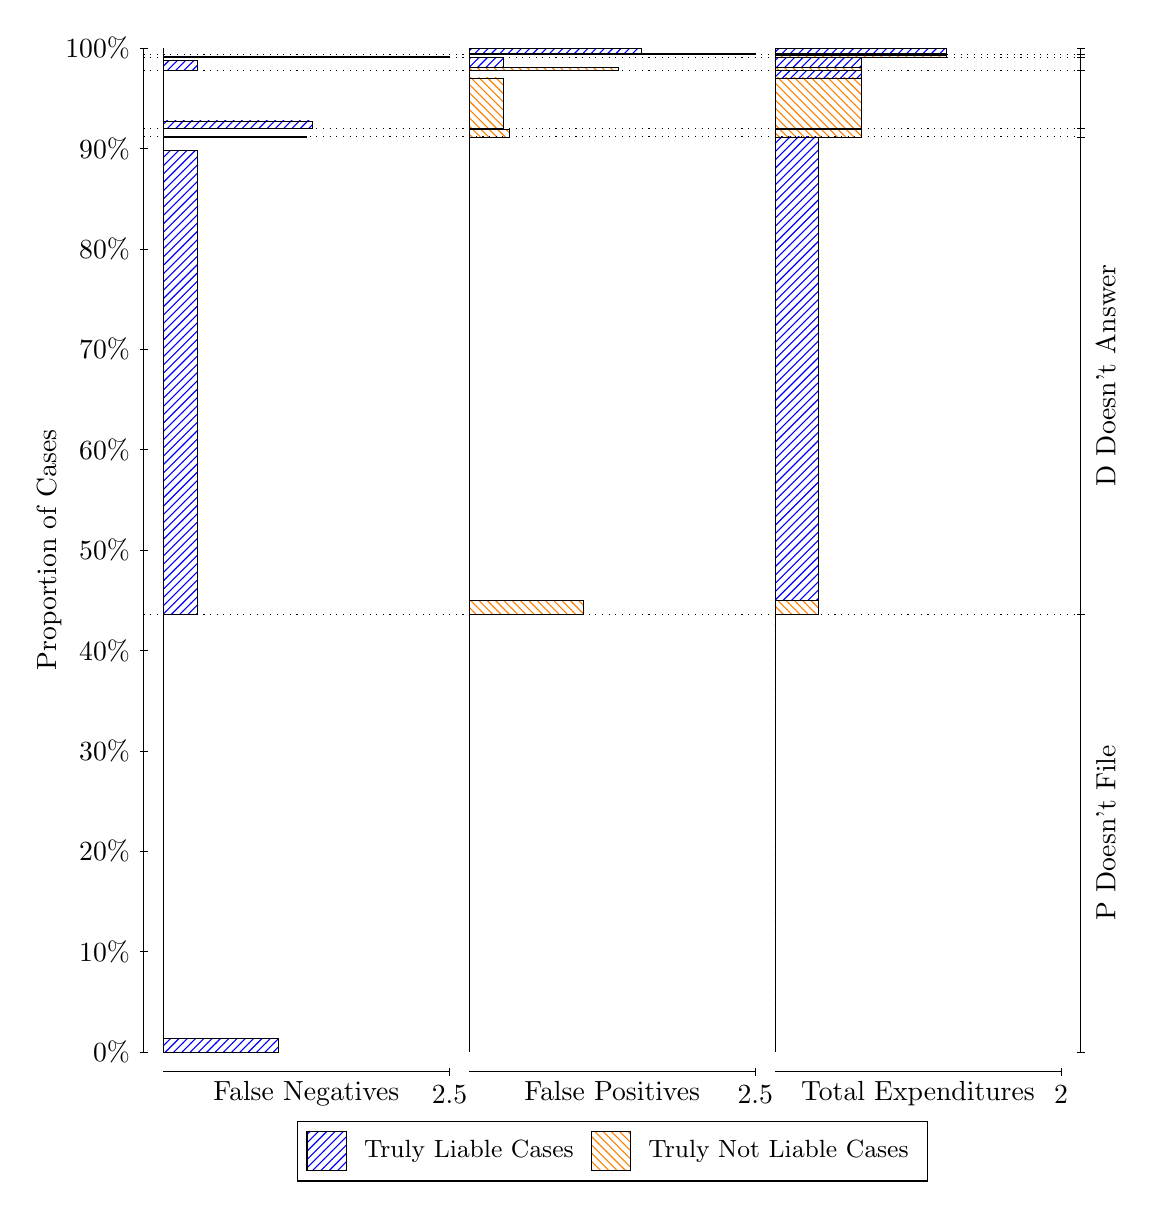
\begin{tikzpicture}
\draw[black, very thin] (1.5,1.75) -- (1.5,14.5);
\node[rotate=90, text=black, anchor=center] at (0.3, 8.125) {Proportion of Cases};
\draw[black, very thin] (1.45,1.75) -- (1.55,1.75);
\node[text=black, anchor=east] at (1.45, 1.75) {0\%};
\draw[black, very thin] (1.45,3.025) -- (1.55,3.025);
\node[text=black, anchor=east] at (1.45, 3.025) {10\%};
\draw[black, very thin] (1.45,4.3) -- (1.55,4.3);
\node[text=black, anchor=east] at (1.45, 4.3) {20\%};
\draw[black, very thin] (1.45,5.575) -- (1.55,5.575);
\node[text=black, anchor=east] at (1.45, 5.575) {30\%};
\draw[black, very thin] (1.45,6.85) -- (1.55,6.85);
\node[text=black, anchor=east] at (1.45, 6.85) {40\%};
\draw[black, very thin] (1.45,8.125) -- (1.55,8.125);
\node[text=black, anchor=east] at (1.45, 8.125) {50\%};
\draw[black, very thin] (1.45,9.4) -- (1.55,9.4);
\node[text=black, anchor=east] at (1.45, 9.4) {60\%};
\draw[black, very thin] (1.45,10.675) -- (1.55,10.675);
\node[text=black, anchor=east] at (1.45, 10.675) {70\%};
\draw[black, very thin] (1.45,11.95) -- (1.55,11.95);
\node[text=black, anchor=east] at (1.45, 11.95) {80\%};
\draw[black, very thin] (1.45,13.225) -- (1.55,13.225);
\node[text=black, anchor=east] at (1.45, 13.225) {90\%};
\draw[black, very thin] (1.45,14.5) -- (1.55,14.5);
\node[text=black, anchor=east] at (1.45, 14.5) {100\%};

\draw[black, very thin] (13.4,1.75) -- (13.4,14.5);
\draw[black, very thin] (13.35,1.75) -- (13.45,1.75);
\node[anchor=west] at (13.35, 1.75) {};
\draw[black, very thin] (13.35,7.3108) -- (13.45,7.3108);
\node[anchor=west] at (13.35, 7.3108) {};
\draw[black, very thin] (13.35,13.371) -- (13.45,13.371);
\node[anchor=west] at (13.35, 13.371) {};
\draw[black, very thin] (13.35,13.475) -- (13.45,13.475);
\node[anchor=west] at (13.35, 13.475) {};
\draw[black, very thin] (13.35,14.22) -- (13.45,14.22);
\node[anchor=west] at (13.35, 14.22) {};
\draw[black, very thin] (13.35,14.381) -- (13.45,14.381);
\node[anchor=west] at (13.35, 14.381) {};
\draw[black, very thin] (13.35,14.421) -- (13.45,14.421);
\node[anchor=west] at (13.35, 14.421) {};
\draw[black, very thin] (13.35,14.5) -- (13.45,14.5);
\node[anchor=west] at (13.35, 14.5) {};

\draw[black, very thin, pattern color=blue, pattern=north east lines] (1.75,1.75) rectangle (3.2033,1.9253);
\draw[black, very thin, pattern color=orange, pattern=north west lines] (1.75,1.9253) rectangle (1.75,7.3108);
\draw[black, very thin, pattern color=blue, pattern=north east lines] (1.75,7.3108) rectangle (2.186,13.196);
\draw[black, very thin, pattern color=orange, pattern=north west lines] (1.75,13.196) rectangle (1.75,13.371);
\draw[black, very thin, pattern color=blue, pattern=north east lines] (1.75,13.371) rectangle (3.5667,13.377);
\draw[black, very thin, pattern color=orange, pattern=north west lines] (1.75,13.377) rectangle (1.75,13.475);
\draw[black, very thin, pattern color=blue, pattern=north east lines] (1.75,13.475) rectangle (3.6393,13.574);
\draw[black, very thin, pattern color=orange, pattern=north west lines] (1.75,13.574) rectangle (1.75,14.22);
\draw[black, very thin, pattern color=blue, pattern=north east lines] (1.75,14.22) rectangle (2.186,14.345);
\draw[black, very thin, pattern color=orange, pattern=north west lines] (1.75,14.345) rectangle (1.75,14.381);
\draw[black, very thin, pattern color=blue, pattern=north east lines] (1.75,14.381) rectangle (5.3833,14.392);
\draw[black, very thin, pattern color=orange, pattern=north west lines] (1.75,14.392) rectangle (1.75,14.421);
\draw[black, very thin, pattern color=orange, pattern=north west lines] (1.75,14.421) rectangle (1.75,14.428);
\draw[black, very thin, pattern color=blue, pattern=north east lines] (1.75,14.428) rectangle (1.75,14.5);
\draw[black, very thin, pattern color=orange, pattern=north west lines] (5.6333,1.75) rectangle (5.6333,7.1355);
\draw[black, very thin, pattern color=blue, pattern=north east lines] (5.6333,7.1355) rectangle (5.6333,7.3108);
\draw[black, very thin, pattern color=orange, pattern=north west lines] (5.6333,7.3108) rectangle (7.0867,7.4861);
\draw[black, very thin, pattern color=blue, pattern=north east lines] (5.6333,7.4861) rectangle (5.6333,13.371);
\draw[black, very thin, pattern color=orange, pattern=north west lines] (5.6333,13.371) rectangle (6.142,13.468);
\draw[black, very thin, pattern color=blue, pattern=north east lines] (5.6333,13.468) rectangle (5.6333,13.475);
\draw[black, very thin, pattern color=orange, pattern=north west lines] (5.6333,13.475) rectangle (6.0693,14.12);
\draw[black, very thin, pattern color=blue, pattern=north east lines] (5.6333,14.12) rectangle (5.6333,14.22);
\draw[black, very thin, pattern color=orange, pattern=north west lines] (5.6333,14.22) rectangle (7.5227,14.255);
\draw[black, very thin, pattern color=blue, pattern=north east lines] (5.6333,14.255) rectangle (6.0693,14.381);
\draw[black, very thin, pattern color=orange, pattern=north west lines] (5.6333,14.381) rectangle (5.6333,14.41);
\draw[black, very thin, pattern color=blue, pattern=north east lines] (5.6333,14.41) rectangle (5.6333,14.421);
\draw[black, very thin, pattern color=orange, pattern=north west lines] (5.6333,14.421) rectangle (9.2667,14.428);
\draw[black, very thin, pattern color=blue, pattern=north east lines] (5.6333,14.428) rectangle (7.8133,14.5);
\draw[black, very thin, pattern color=orange, pattern=north west lines] (9.5167,1.75) rectangle (9.5167,7.1355);
\draw[black, very thin, pattern color=blue, pattern=north east lines] (9.5167,7.1355) rectangle (9.5167,7.3108);
\draw[black, very thin, pattern color=orange, pattern=north west lines] (9.5167,7.3108) rectangle (10.062,7.4861);
\draw[black, very thin, pattern color=blue, pattern=north east lines] (9.5167,7.4861) rectangle (10.062,13.371);
\draw[black, very thin, pattern color=orange, pattern=north west lines] (9.5167,13.371) rectangle (10.607,13.468);
\draw[black, very thin, pattern color=blue, pattern=north east lines] (9.5167,13.468) rectangle (10.607,13.475);
\draw[black, very thin, pattern color=orange, pattern=north west lines] (9.5167,13.475) rectangle (10.607,14.12);
\draw[black, very thin, pattern color=blue, pattern=north east lines] (9.5167,14.12) rectangle (10.607,14.22);
\draw[black, very thin, pattern color=orange, pattern=north west lines] (9.5167,14.22) rectangle (10.607,14.255);
\draw[black, very thin, pattern color=blue, pattern=north east lines] (9.5167,14.255) rectangle (10.607,14.381);
\draw[black, very thin, pattern color=orange, pattern=north west lines] (9.5167,14.381) rectangle (11.697,14.41);
\draw[black, very thin, pattern color=blue, pattern=north east lines] (9.5167,14.41) rectangle (11.697,14.421);
\draw[black, very thin, pattern color=orange, pattern=north west lines] (9.5167,14.421) rectangle (11.697,14.428);
\draw[black, very thin, pattern color=blue, pattern=north east lines] (9.5167,14.428) rectangle (11.697,14.5);
\draw[black, dotted] (1.5,7.3108) -- (13.4,7.3108);
\draw[black, dotted] (1.5,13.371) -- (13.4,13.371);
\draw[black, dotted] (1.5,13.475) -- (13.4,13.475);
\draw[black, dotted] (1.5,14.22) -- (13.4,14.22);
\draw[black, dotted] (1.5,14.381) -- (13.4,14.381);
\draw[black, dotted] (1.5,14.421) -- (13.4,14.421);
\draw[black, very thin] (1.75,1.5) -- (5.3833,1.5);
\node[text=black, anchor=north] at (3.5667, 1.5) {False Negatives};
\draw[black, very thin] (5.3833,1.45) -- (5.3833,1.55);
\node[text=black, anchor=north] at (5.3833, 1.45) {2.5};

\draw[black, very thin] (5.6333,1.5) -- (9.2667,1.5);
\node[text=black, anchor=north] at (7.45, 1.5) {False Positives};
\draw[black, very thin] (9.2667,1.45) -- (9.2667,1.55);
\node[text=black, anchor=north] at (9.2667, 1.45) {2.5};

\draw[black, very thin] (9.5167,1.5) -- (13.15,1.5);
\node[text=black, anchor=north] at (11.333, 1.5) {Total Expenditures};
\draw[black, very thin] (13.15,1.45) -- (13.15,1.55);
\node[text=black, anchor=north] at (13.15, 1.45) {2};

\node[text=black, centered, rotate=90] at (13.72, 4.5304) {P Doesn't File};
\node[text=black, centered, rotate=90] at (13.72, 10.341) {D Doesn't Answer};






\draw (7.449999999999999,1.5) node[draw=none] (baseCoordinate) {};
\begin{scope}[align=center]
        \matrix[scale=0.5, draw=black, below=0.5cm of baseCoordinate, nodes={draw}, column sep=0.1cm]{
            \node[rectangle, draw, minimum width=0.5cm, minimum height=0.5cm, pattern color=blue, pattern=north east lines] {}; &
            \node[draw=none, font=\small, text=black] (B) {Truly Liable Cases}; &
            \node[rectangle, draw, minimum width=0.5cm, minimum height=0.5cm, pattern color=orange, pattern=north west lines] {}; &
            \node[draw=none, font=\small, text=black] (B) {Truly Not Liable Cases}; \\
            };
\end{scope}

\end{tikzpicture}
\end{document}